\subsection{Softwaresysteme}
Mit Software wird die Kommunikation zwischen externer Steuerungseinheit und Ballwurfmaschine, die Ortung des Korbes, sowie deren Konfiguration und die Steuerung der Motoren umgesetzt. In den folgenden Kapitel werden auf die einzelnen Komponenten eingegangen.

\subsubsection{Ortung des Korbes}
Der Ort des Korbes wird optisch bestimmt. Dazu wird zu Beginn des Prozesses ein Foto mittels der Raspberry Pi Kamera geschossen. Dieses Bild wird anschliessend auf dem Raspberry Pi mittels eines Algorithmus analysiert.\\
\\
\textbf{Algorithmus zur Ortung des Korbes}\\
\label{abb-algorithmus-zur-ortung-des-korbes}
Die grössten Herausforderungen stellen die unterschiedlichen Lichtverhältnisse dar. Der Algorithmus muss so robust sein, dass dieser damit umgehen kann. Generell sind mit Scheinwerfer von oben zu rechnen wobei der Korb so einen Schatten erhält. Auch Licht von der Seite durch die Fenster kann die Lichtverhältnisse beeinflussen.\\
\\
\textbf{Ablauf des Algorithmus}
\begin{figure}[h!]
	\centering
	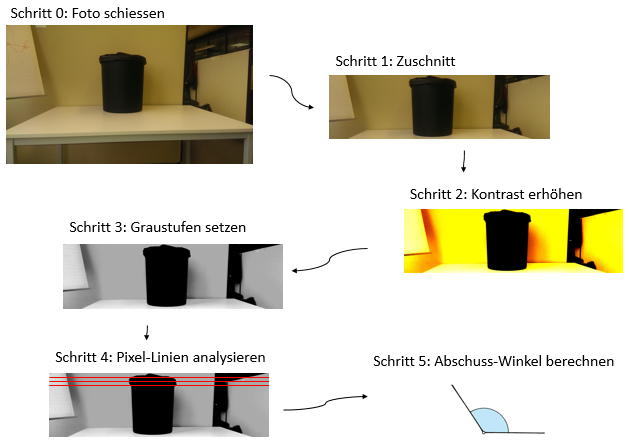
\includegraphics[scale=0.75]{../../fig/ablauf-ortung-des-korbes-algorithmus.png}
	\caption{Ablauf des Algorithmus}
\end{figure}

\textbf{Parameter des Algorithmus}\\
Der Algorithmus erwartet nachfolgende Parameter um seine Arbeit erfolgreich zu verrichten. Diese Parameter sind das Ergebnis aus gemachten Tests, welche im Anhang \ref{anhang-versuche-tests} zu finden sind.
\begin{itemize}
	\item Qualität. Die höchste Qualität des Bildes wird nicht benötigt. Dies würde nur unnötig den Speicherbedarfs des Bildes erhöhen und somit längere Übertragungs- und Verarbeitungsdauern verursachen. 
	\item ROI (region of interest): Der Ausschnitt des Bildes wird dadurch definiert.
	\item Kontrast: Für das Strecken des Histogrammes.
	\item Graustufen: Für die vereinfachte Auswertung des Pixel-Linien.
	\item Pixel Linie: Zu analysierende Pixel-Linie.
\end{itemize}
Auf die einzelnen Parameter wird in der Beschreibung des Ablaufes eingegangen. Gemäss Tests sollten diese Parameter für eine erfolgreiche Detektierung reichen. Jedoch wird eine Auge auf die Helligkeitseinstellung sowie den Weissabgleich geworfen. Diese Punkte sind nicht zu vernachlässigen nach Aussagen eines Fotografie-Experten (M. Vogel).\\
\\
Auf der Abbildung sind die einzelnen Schritte zu erkennen, welche auf das Foto angewendet werden. Nachfolgend werden diese Schritte genauer erläutert:
\begin{itemize}
	\item Schritt 0 - Foto schiessen: Mit der Raspberry Pi Kamera wird ein Foto gemacht.
	
	\item Schritt 1 - Zuschneiden: Das Bild wird zugeschnitten. Irrelevante Informationen können so bereits eliminiert werden. Ausserdem hat es den positiven Effekt, dass das Bild physisch kleiner wird. Weitere Verarbeitungsschritte müssen so weniger Ressourcen aufwenden. 
	
	\item Schritt 2 - Kontrast verstärken: In diesem Schritt wird der Kontrast des Bildes erhöht. Das Histogramm verbreitert sich und helle Punkte werden noch heller und dunkle Punkte noch dunkler. Sprich der schwarze Korb wird noch intensiver erkennbar. 
	
	\item Schritt 3 - Graustufen setzen: Das Bild wird in Graustufen konvertiert. Dies hat zur Folge, dass jedes Pixel im Bild jeweils einen gleich hohen Anteil an rot, blau und grün Werten hält. Tiefe Werte bedeuten, dass der Punkt dunkel ist, hohe Werte entsprechend hell. (RGB(0,0,0) = schwarz, RGB(255,255,255) = weiss).
	
	\item Schritt 4 - Pixel analysieren: Es werden mehrere Linie auf dem Bild analysiert. Nun ist auf diesen Linien ein längerer Bereich recht dunkel im Verhältnis zu den anderen Bereichen. Da kann nun angenommen werden, dass dort der Korb ist. Um das Problem mit dem Schatten zu umgehen, wird eine Linie analysiert welche möglichst weit oben im Bild ist, denn die Schatten könnten den Korb unten künstlich verbreitern. Um ein exakteres Resultat zu erhalten und dem Algorithmus mehr Robustheit zu gewähren, werden mehrere Linien analysiert und der Mittelwert aus allen analysierten Linien genommen. So umgeht man die Problematik einer Linie, welche aus irgendeinem Grund überhaupt nicht dem Muster entspricht.
	
	\item Schritt 5 - Abschuss-Winkel berechnen: Sobald der Punkt des Korbes auf dem Bild bekannt ist, kann der physische Ort bestimmt werden. Da die Kamera immer am gleichen Ort ist und der Zuschnitt des Bildes gleich erfolgt, kann eine Mapping-Tabelle dafür verwendet werden. In dieser Tabelle findet man die Zuweisung des Bild-Punktes zu dem physischen Ort. Als Output erzeugt der Algorithmus den Winkel zwischen Korb und Kamera.
\end{itemize} 
Die Raspberry Pi Kamera kann bereits einige Schritte gleich selbst durchführen. Dazu zählen Schritt 1, 2 und 3 (siehe Abschnitt \ref{subsub:raspistill}). Das bedeutet, dass der Algorithmus sich selbst nicht um diese Transformationen kümmern muss. Er muss lediglich diese Parameter der Kamera weiterreichen.\\
\\
Die Schritte 4 und 5 müssen jedoch auf dem Raspberry Pi implementiert werden.

\begin{lstlisting}[language=Python,caption={Pixel aus einem Bild auslesen mit Python},label=lst:image_python]
from PIL import Image
bild = Image.open('korb.jpg')
pixelarray = bild.load()
pixelarray[10,10] = (0,0,0)
print (pixelarray[10,10])
\end{lstlisting}

Auf der Auflistung \ref{lst:image_python} ist zu erkennen, wie man ein Pixel auslesen kann.\\
\\
Alle Parameter für die einzelnen Schritte des Algorithmus müssen konfigurierbar sein. Beim Einrichten der Ballwurfmaschine dürfen fünf Minuten verwendet werden. In dieser Zeit sollen diese Parameter der Umgebung angepasst werden können (siehe Abschnitt \ref{ss-config-paramater-ortung-orb}).\\
\\
\textbf{Implementierung}\\
Die Implementation erfolgt in Python auf dem Raspberry Pi. Python ist bewährt und bietet viele Bibliotheken. Verwendet wird die Version 2. Version 3 wurde seit langem veröffentlicht, konnte sich jedoch noch nicht endgültig durchsetzen. Viele Bibliotheken wurden noch immer nicht portiert. Zur Verwendung kommt die Bibliothek \verb|Pillow| mit welchem man simple Bildoperationen durchführen kann. Um die Kamera anzusteuern wird die Bibliothek \verb|Picamera|.

\subsubsection{Ballwurfmaschine-UI}
\label{ss-config-paramater-ortung-orb}
Damit die Parameter des Algorithmus für die Ortung des Korbes (siehe Abschnitt \ref{abb-algorithmus-zur-ortung-des-korbes}) angepasst werden können, wird eine Software auf Seite der externen Steuerungseinheit implementiert. Diese Komponente besitzt ein UI (grafische Benutzeroberfläche bzw. User-Interface), welches in Java programmiert wird.

\begin{figure}[h!]
	\centering
	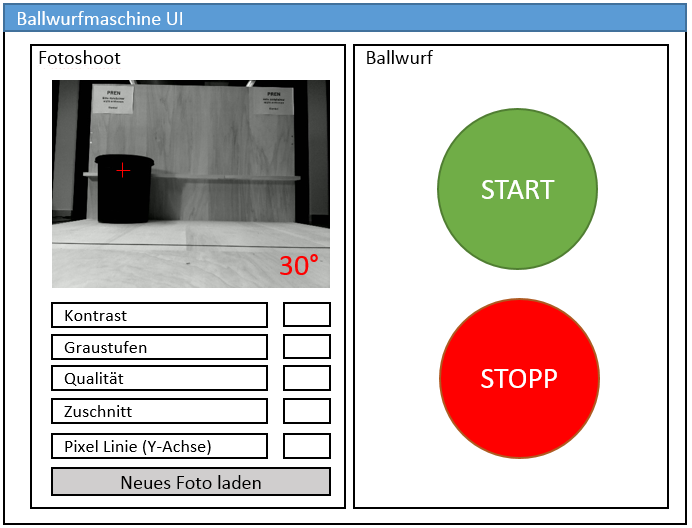
\includegraphics[scale=0.75]{../../fig/fotoshoot-configurator.png}
	\caption{Ballwurfmaschine-UI Skizze}
\end{figure}

Das UI der Ballwurfmaschine lässt im Bereich Fotoshoot alle relevanten Werte konfigurieren. Es erhält jeweils das aktuelle Foto, welches in diesem Prozess mit Informationen angereichert wird. Der Algorithmus markiert den Korb mit einem Fadenkreuz und schreibt den Winkel unten rechts aufs Bild.

\subsubsection{Steuerung der Motoren}
Die Motoransteuerung findet kaskadiert statt, über zwei Abstraktionslayer
wie in der Abbildung \ref{fig:motor-control-overview} und 
\ref{fig:kontextdiagramm} dargestellt. Die Ansteuerung erfolgt zunächst
beim Raspberry Pi auf dem obersten Layer. Dieser hat eine UART
Schnittstelle zur Verfügung zum Freedomboard, auf welcher mittels
einfachen Kommandos die Motoren angesteuert werden. 

Auf dem zweiten Layer befindet sich das Freedomboard, welches die über UART
eingegebenen Kommandos weiterverarbeitet. Hierfür ist ein Zustandsautomat
implementiert, welcher die UART Schnittstelle bedient und die Befehle
verarbeitet.

Die eingespielten Kommandos werden mit diesem Zustandsautomat verarbeitet und
den einzelnen Motorentreibern zugespielt. Diese Treiber, falls vorhanden,
bilden den untersten Layer der Ansteuerung. Diese Treiber sind entweder
direkt durch das Freedomboard gesteuert (z.B. mit PWM-Signalen) oder 
parametrierbar über standardisierte Schnittstellen wie SPI oder I$^2$C.

\begin{figure}[h!]
	\centering
	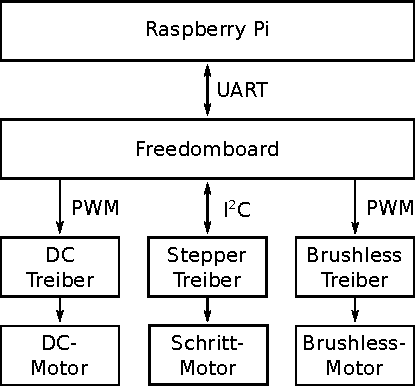
\includegraphics[scale=1]{../../fig/motor-control-overview.pdf}
	\caption{Schnittstellenübersicht der Motoransteuerung}
	\label{fig:motor-control-overview}
\end{figure}

Die Software auf dem Freedomboard wird in der Programmiersprache C
implementiert. Als Entwicklungshilfe stehen zwei Entwicklungsumgebungen
des Herstellers Freescale Semicondutor zur Verfügung, einerseits CodeWarrior
und andererseits KinetisDesignStudio. Beide Entwicklungsumgebungen sind
an der Hochschule Luzern in Gebrauch und verfügbar für die Benutzung.

